\documentclass[]{article}
\usepackage{lmodern}
\usepackage{amssymb,amsmath}
\usepackage{ifxetex,ifluatex}
\usepackage{fixltx2e} % provides \textsubscript
\ifnum 0\ifxetex 1\fi\ifluatex 1\fi=0 % if pdftex
  \usepackage[T1]{fontenc}
  \usepackage[utf8]{inputenc}
\else % if luatex or xelatex
  \ifxetex
    \usepackage{mathspec}
  \else
    \usepackage{fontspec}
  \fi
  \defaultfontfeatures{Ligatures=TeX,Scale=MatchLowercase}
\fi
% use upquote if available, for straight quotes in verbatim environments
\IfFileExists{upquote.sty}{\usepackage{upquote}}{}
% use microtype if available
\IfFileExists{microtype.sty}{%
\usepackage{microtype}
\UseMicrotypeSet[protrusion]{basicmath} % disable protrusion for tt fonts
}{}
\usepackage[margin=1in]{geometry}
\usepackage{hyperref}
\hypersetup{unicode=true,
            pdftitle={Homework 11},
            pdfauthor={Emorie Beck},
            pdfborder={0 0 0},
            breaklinks=true}
\urlstyle{same}  % don't use monospace font for urls
\usepackage{color}
\usepackage{fancyvrb}
\newcommand{\VerbBar}{|}
\newcommand{\VERB}{\Verb[commandchars=\\\{\}]}
\DefineVerbatimEnvironment{Highlighting}{Verbatim}{commandchars=\\\{\}}
% Add ',fontsize=\small' for more characters per line
\usepackage{framed}
\definecolor{shadecolor}{RGB}{248,248,248}
\newenvironment{Shaded}{\begin{snugshade}}{\end{snugshade}}
\newcommand{\KeywordTok}[1]{\textcolor[rgb]{0.13,0.29,0.53}{\textbf{#1}}}
\newcommand{\DataTypeTok}[1]{\textcolor[rgb]{0.13,0.29,0.53}{#1}}
\newcommand{\DecValTok}[1]{\textcolor[rgb]{0.00,0.00,0.81}{#1}}
\newcommand{\BaseNTok}[1]{\textcolor[rgb]{0.00,0.00,0.81}{#1}}
\newcommand{\FloatTok}[1]{\textcolor[rgb]{0.00,0.00,0.81}{#1}}
\newcommand{\ConstantTok}[1]{\textcolor[rgb]{0.00,0.00,0.00}{#1}}
\newcommand{\CharTok}[1]{\textcolor[rgb]{0.31,0.60,0.02}{#1}}
\newcommand{\SpecialCharTok}[1]{\textcolor[rgb]{0.00,0.00,0.00}{#1}}
\newcommand{\StringTok}[1]{\textcolor[rgb]{0.31,0.60,0.02}{#1}}
\newcommand{\VerbatimStringTok}[1]{\textcolor[rgb]{0.31,0.60,0.02}{#1}}
\newcommand{\SpecialStringTok}[1]{\textcolor[rgb]{0.31,0.60,0.02}{#1}}
\newcommand{\ImportTok}[1]{#1}
\newcommand{\CommentTok}[1]{\textcolor[rgb]{0.56,0.35,0.01}{\textit{#1}}}
\newcommand{\DocumentationTok}[1]{\textcolor[rgb]{0.56,0.35,0.01}{\textbf{\textit{#1}}}}
\newcommand{\AnnotationTok}[1]{\textcolor[rgb]{0.56,0.35,0.01}{\textbf{\textit{#1}}}}
\newcommand{\CommentVarTok}[1]{\textcolor[rgb]{0.56,0.35,0.01}{\textbf{\textit{#1}}}}
\newcommand{\OtherTok}[1]{\textcolor[rgb]{0.56,0.35,0.01}{#1}}
\newcommand{\FunctionTok}[1]{\textcolor[rgb]{0.00,0.00,0.00}{#1}}
\newcommand{\VariableTok}[1]{\textcolor[rgb]{0.00,0.00,0.00}{#1}}
\newcommand{\ControlFlowTok}[1]{\textcolor[rgb]{0.13,0.29,0.53}{\textbf{#1}}}
\newcommand{\OperatorTok}[1]{\textcolor[rgb]{0.81,0.36,0.00}{\textbf{#1}}}
\newcommand{\BuiltInTok}[1]{#1}
\newcommand{\ExtensionTok}[1]{#1}
\newcommand{\PreprocessorTok}[1]{\textcolor[rgb]{0.56,0.35,0.01}{\textit{#1}}}
\newcommand{\AttributeTok}[1]{\textcolor[rgb]{0.77,0.63,0.00}{#1}}
\newcommand{\RegionMarkerTok}[1]{#1}
\newcommand{\InformationTok}[1]{\textcolor[rgb]{0.56,0.35,0.01}{\textbf{\textit{#1}}}}
\newcommand{\WarningTok}[1]{\textcolor[rgb]{0.56,0.35,0.01}{\textbf{\textit{#1}}}}
\newcommand{\AlertTok}[1]{\textcolor[rgb]{0.94,0.16,0.16}{#1}}
\newcommand{\ErrorTok}[1]{\textcolor[rgb]{0.64,0.00,0.00}{\textbf{#1}}}
\newcommand{\NormalTok}[1]{#1}
\usepackage{graphicx,grffile}
\makeatletter
\def\maxwidth{\ifdim\Gin@nat@width>\linewidth\linewidth\else\Gin@nat@width\fi}
\def\maxheight{\ifdim\Gin@nat@height>\textheight\textheight\else\Gin@nat@height\fi}
\makeatother
% Scale images if necessary, so that they will not overflow the page
% margins by default, and it is still possible to overwrite the defaults
% using explicit options in \includegraphics[width, height, ...]{}
\setkeys{Gin}{width=\maxwidth,height=\maxheight,keepaspectratio}
\IfFileExists{parskip.sty}{%
\usepackage{parskip}
}{% else
\setlength{\parindent}{0pt}
\setlength{\parskip}{6pt plus 2pt minus 1pt}
}
\setlength{\emergencystretch}{3em}  % prevent overfull lines
\providecommand{\tightlist}{%
  \setlength{\itemsep}{0pt}\setlength{\parskip}{0pt}}
\setcounter{secnumdepth}{0}
% Redefines (sub)paragraphs to behave more like sections
\ifx\paragraph\undefined\else
\let\oldparagraph\paragraph
\renewcommand{\paragraph}[1]{\oldparagraph{#1}\mbox{}}
\fi
\ifx\subparagraph\undefined\else
\let\oldsubparagraph\subparagraph
\renewcommand{\subparagraph}[1]{\oldsubparagraph{#1}\mbox{}}
\fi

%%% Use protect on footnotes to avoid problems with footnotes in titles
\let\rmarkdownfootnote\footnote%
\def\footnote{\protect\rmarkdownfootnote}

%%% Change title format to be more compact
\usepackage{titling}

% Create subtitle command for use in maketitle
\newcommand{\subtitle}[1]{
  \posttitle{
    \begin{center}\large#1\end{center}
    }
}

\setlength{\droptitle}{-2em}
  \title{Homework 11}
  \pretitle{\vspace{\droptitle}\centering\huge}
  \posttitle{\par}
\subtitle{Psych 5068}
  \author{Emorie Beck}
  \preauthor{\centering\large\emph}
  \postauthor{\par}
  \predate{\centering\large\emph}
  \postdate{\par}
  \date{\today}

\usepackage{fancyhdr}
\usepackage{array}
\usepackage{longtable}
\usepackage{lscape}
\newcommand{\blandscape}{\begin{landscape}}
\newcommand{\elandscape}{\end{landscape}}
\usepackage{dcolumn}
\usepackage{bbm}
\usepackage{threeparttable}
\usepackage{booktabs}
\usepackage{expex}
\usepackage{pdflscape}
\usepackage{rotating, graphicx}
\usepackage{tabulary}
\usepackage{lscape}
\usepackage{makecell}
\usepackage{algorithm}
\usepackage{multirow}
\usepackage{colortbl}
\usepackage{longtable}
\usepackage{array}
\usepackage{multirow}
\usepackage{wrapfig}
\usepackage{float}
\usepackage{pdflscape}
\usepackage{tabu}
\usepackage{threeparttable}
\usepackage{booktabs}
\usepackage{longtable}
\usepackage{array}
\usepackage{multirow}
\usepackage[table]{xcolor}
\usepackage{wrapfig}
\usepackage{float}
\usepackage{colortbl}
\usepackage{pdflscape}
\usepackage{tabu}
\usepackage{threeparttable}
\usepackage[normalem]{ulem}

\begin{document}
\maketitle

{
\setcounter{tocdepth}{2}
\tableofcontents
}
\section{Workspace}\label{workspace}

\subsection{Packages}\label{packages}

\subsection{Data}\label{data}

\begin{Shaded}
\begin{Highlighting}[]
\KeywordTok{source}\NormalTok{(}\StringTok{"https://raw.githubusercontent.com/emoriebeck/homeworks/master/table_fun.R"}\NormalTok{)}
\NormalTok{data_url <-}\StringTok{ "https://raw.githubusercontent.com/emoriebeck/homeworks/master/homework11/Safety_Binary(2).csv"}
\NormalTok{dat      <-}\StringTok{ }\NormalTok{data_url }\OperatorTok\StringTok{ }\NormalTok{read.csv }\OperatorTok\StringTok{ }\NormalTok{tbl_df }
\end{Highlighting}
\end{Shaded}

Level 1:\\
\(\eta_{ij} = \beta_{0j} + \beta_{1j}*GMC\_Age + \beta_{2j}*sex\)

Level 2:\\
\(\beta_{0j} = \gamma_{00} + \gamma_{01}*crowded\_GMC_j + \gamma_{02}*economic_j + u_{0j}\)\\
\(\beta_{1j} = \gamma_{10} + \gamma_{11}*crowded\_GMC_j + \gamma_{12}*economic_j + u_{1j}\)\\
\(\beta_{2j} = \gamma_{20} + \gamma_{21}*crowded\_GMC_j + \gamma_{22}*economic_j\)

For this assignment you will extend these analyses to test nonlinearity
and interactions. The data for this assignment are contained in the
file, Safety\_Binary.csv.

If you have problems getting some of the models to converge, you can try
alternative optimizers and increase the number of iterations that are
used before the algorithm gives up. The easiest way to do this is to
create several alternative control lists and then substitute them into
the model statement as needed:

\begin{Shaded}
\begin{Highlighting}[]
\NormalTok{cl1 <-}\StringTok{ }\KeywordTok{glmerControl}\NormalTok{(}\DataTypeTok{optimizer =} \StringTok{"bobyqa"}\NormalTok{, }\DataTypeTok{optCtrl=}\KeywordTok{list}\NormalTok{(}\DataTypeTok{maxfun=}\DecValTok{10000}\NormalTok{))}
\NormalTok{cl2 <-}\StringTok{ }\KeywordTok{glmerControl}\NormalTok{(}\DataTypeTok{optimizer =} \StringTok{"Nelder_Mead"}\NormalTok{, }\DataTypeTok{optCtrl=}\KeywordTok{list}\NormalTok{(}\DataTypeTok{maxfun=}\DecValTok{10000}\NormalTok{))}
\NormalTok{cl3 <-}\StringTok{ }\KeywordTok{glmerControl}\NormalTok{(}\DataTypeTok{optimizer =} \StringTok{"optimx"}\NormalTok{,}\DataTypeTok{optCtrl=}\KeywordTok{list}\NormalTok{(}\DataTypeTok{method=}\StringTok{"nlminb"}\NormalTok{,}\DataTypeTok{maxiter=}\DecValTok{10000}\NormalTok{))}
\end{Highlighting}
\end{Shaded}

You will need the \texttt{optimx} package for the last one.\\
Switch to a different optimizer like this:

\texttt{Safety\textbackslash{}\_Fit\textbackslash{}\_1\ \textless{}-\ glmer(unsafe\ \textasciitilde{}\ 1\ +\ Z\textbackslash{}\_Age\ +\ Z\textbackslash{}\_Age\textbackslash{}\_SQ\ +\ sex\ +\ (1\ +\ Z\textbackslash{}\_Age\ +\ Z\textbackslash{}\_Age\textbackslash{}\_SQ\ +\ sex\textbar{}street),\ data=Safety\textbackslash{}\_Data,\ binomial("logit"),\ control=cl1)}

\section{Question 1}\label{question-1}

In the data file, two of the variables are named age and crowded.
Standardize them and name them Z\_Age and Z\_Crowded. Create a new
variable that is the square of Z\_Age; name it Z\_Age\_SQ.

\begin{Shaded}
\begin{Highlighting}[]
\NormalTok{dat <-}\StringTok{ }\NormalTok{dat }\OperatorTok
\StringTok{  }\KeywordTok{mutate_at}\NormalTok{(}\KeywordTok{vars}\NormalTok{(age, crowded), }\KeywordTok{funs}\NormalTok{(}\DataTypeTok{z =} \KeywordTok{as.numeric}\NormalTok{(}\KeywordTok{scale}\NormalTok{(.)))) }\OperatorTok
\StringTok{  }\KeywordTok{rename}\NormalTok{(}\DataTypeTok{Z_Age =}\NormalTok{ age_z, }\DataTypeTok{Z_Crowded =}\NormalTok{ crowded_z) }\OperatorTok
\StringTok{  }\KeywordTok{mutate}\NormalTok{(}\DataTypeTok{Z_Age_SQ =}\NormalTok{ Z_Age}\OperatorTok{^}\DecValTok{2}\NormalTok{)}
\end{Highlighting}
\end{Shaded}

\section{Question 2}\label{question-2}

Test a Level 1 model that contains Z\_Age, Z\_Age\_SQ, and sex. Level 2
should be unconditional (no predictors) with all residual variances
estimated.

\begin{Shaded}
\begin{Highlighting}[]
\NormalTok{fit1 <-}\StringTok{ }\KeywordTok{glmer}\NormalTok{(unsafe }\OperatorTok{~}\StringTok{ }\NormalTok{Z_Age }\OperatorTok{+}\StringTok{ }\NormalTok{Z_Age_SQ }\OperatorTok{+}\StringTok{ }\NormalTok{sex }\OperatorTok{+}\StringTok{ }\NormalTok{(Z_Age }\OperatorTok{+}\StringTok{ }\NormalTok{Z_Age_SQ }\OperatorTok{+}\StringTok{ }\NormalTok{sex }\OperatorTok{|}\StringTok{ }\NormalTok{street), }
              \DataTypeTok{data =}\NormalTok{ dat, }\DataTypeTok{family =} \KeywordTok{binomial}\NormalTok{(}\StringTok{"logit"}\NormalTok{), }\DataTypeTok{control=}\NormalTok{cl1)}
\NormalTok{tab1 <-}\StringTok{ }\KeywordTok{table_fun}\NormalTok{(fit1)}

\NormalTok{tab1 }\OperatorTok
\StringTok{  }\KeywordTok{select}\NormalTok{(}\OperatorTok{-}\NormalTok{type) }\OperatorTok
\StringTok{  }\KeywordTok{kable}\NormalTok{(., }\StringTok{"latex"}\NormalTok{, }\DataTypeTok{booktabs =}\NormalTok{ T, }\DataTypeTok{escape =}\NormalTok{ F,}
        \DataTypeTok{col.names =} \KeywordTok{c}\NormalTok{(}\StringTok{""}\NormalTok{, }\StringTok{"b"}\NormalTok{, }\StringTok{"OR"}\NormalTok{, }\StringTok{"CI"}\NormalTok{)) }\OperatorTok
\StringTok{  }\KeywordTok{kable_styling}\NormalTok{(}\DataTypeTok{full_width =}\NormalTok{ F) }\OperatorTok
\StringTok{  }\KeywordTok{group_rows}\NormalTok{(}\StringTok{"Fixed"}\NormalTok{, }\DecValTok{1}\NormalTok{,}\DecValTok{4}\NormalTok{) }\OperatorTok
\StringTok{  }\KeywordTok{group_rows}\NormalTok{(}\StringTok{"Random"}\NormalTok{, }\DecValTok{5}\NormalTok{,}\DecValTok{8}\NormalTok{) }\OperatorTok
\StringTok{  }\KeywordTok{group_rows}\NormalTok{(}\StringTok{"Model"}\NormalTok{, }\DecValTok{9}\NormalTok{,}\DecValTok{10}\NormalTok{)}
\end{Highlighting}
\end{Shaded}

\begin{table}[H]
\centering
\begin{tabular}{llll}
\toprule
 & b & OR & CI\\
\midrule
\addlinespace[0.3em]
\multicolumn{4}{l}{\textbf{Fixed}}\\
\hspace{1em}Intercept & -0.64 & 0.53 & [0.36, 0.73]\\
\hspace{1em}Z\_Age & 0.77 & 2.16 & [1.62, 3.02]\\
\hspace{1em}Z\_Age\_SQ & 0.11 & 1.11 & [0.96, 1.46]\\
\hspace{1em}sex & 1.07 & 2.92 & [2.03, 4.17]\\
\addlinespace[0.3em]
\multicolumn{4}{l}{\textbf{Random}}\\
\hspace{1em}$\tau_{00}$ & 0.85 & 2.35 & [1.42, 8.32]\\
\hspace{1em}$\tau_{11}$ & 0.50 & 1.66 & [1.05, 2.66]\\
\hspace{1em}$\tau_{22}$ & 0.13 & 1.14 & [1.01, 1.70]\\
\hspace{1em}$\tau_{33}$ & 0.56 & 1.75 & [1.05, 2.87]\\
$R^2_m$ & 0.14 & 1.15 & [, ]\\
$R^2_c$ & 0.47 & 1.60 & [, ]\\
\bottomrule
\end{tabular}
\end{table}

\subsection{Part A}\label{part-a}

Is there a nonlinear relationship between age and feeling unsafe?\\
No, there is no nonlinear relationship between Age and feeling unsafe
(b = 0.11, OR = 1.11, 95\% CI = {[}0.96, 1.46{]}).

\subsection{Part B}\label{part-b}

Is sex still a significant predictor?\\
Sex is still a significant preditor of feeling unsafe (b = 1.07, OR =
2.92, 95\% CI = {[}2.03, 4.17{]}). The odds of a woman feeling unsafe is
2.92 times higher than a man, on average.

\subsection{Part C}\label{part-c}

Can this model be simplified by eliminating any Level 2 variances? Test
the following simplifications (the intercept is retained in all random
effects specifications):

\subsubsection{Part i}\label{part-i}

Eliminate Z\_Age\_SQ from the random effects.

\begin{Shaded}
\begin{Highlighting}[]
\NormalTok{fit1i <-}\StringTok{ }\KeywordTok{glmer}\NormalTok{(unsafe }\OperatorTok{~}\StringTok{ }\NormalTok{Z_Age }\OperatorTok{+}\StringTok{ }\NormalTok{Z_Age_SQ }\OperatorTok{+}\StringTok{ }\NormalTok{sex }\OperatorTok{+}\StringTok{ }\NormalTok{(Z_Age }\OperatorTok{+}\StringTok{ }\NormalTok{sex }\OperatorTok{|}\StringTok{ }\NormalTok{street), }
               \DataTypeTok{data =}\NormalTok{ dat, }\DataTypeTok{family =} \KeywordTok{binomial}\NormalTok{(}\StringTok{"logit"}\NormalTok{), }\DataTypeTok{control=}\NormalTok{cl1)}
\NormalTok{tab1i <-}\StringTok{ }\KeywordTok{table_fun}\NormalTok{(fit1i)}
\end{Highlighting}
\end{Shaded}

\subsubsection{Part ii}\label{part-ii}

Eliminate Z\_Age and Z\_Age\_SQ from the random effects.

\begin{Shaded}
\begin{Highlighting}[]
\NormalTok{fit1ii <-}\StringTok{ }\KeywordTok{glmer}\NormalTok{(unsafe }\OperatorTok{~}\StringTok{ }\NormalTok{Z_Age }\OperatorTok{+}\StringTok{ }\NormalTok{Z_Age_SQ }\OperatorTok{+}\StringTok{ }\NormalTok{sex }\OperatorTok{+}\StringTok{ }\NormalTok{(sex }\OperatorTok{|}\StringTok{ }\NormalTok{street), }
                \DataTypeTok{data =}\NormalTok{ dat, }\DataTypeTok{family =} \KeywordTok{binomial}\NormalTok{(}\StringTok{"logit"}\NormalTok{))}
\NormalTok{tab1ii <-}\StringTok{ }\KeywordTok{table_fun}\NormalTok{(fit1ii)}
\end{Highlighting}
\end{Shaded}

\subsubsection{Part iii}\label{part-iii}

Eliminate sex from the random effects.

\begin{Shaded}
\begin{Highlighting}[]
\NormalTok{fit1iii <-}\StringTok{ }\KeywordTok{glmer}\NormalTok{(unsafe }\OperatorTok{~}\StringTok{ }\NormalTok{Z_Age }\OperatorTok{+}\StringTok{ }\NormalTok{Z_Age_SQ }\OperatorTok{+}\StringTok{ }\NormalTok{sex }\OperatorTok{+}\StringTok{ }\NormalTok{(Z_Age }\OperatorTok{+}\StringTok{ }\NormalTok{Z_Age_SQ }\OperatorTok{|}\StringTok{ }\NormalTok{street), }
                 \DataTypeTok{data =}\NormalTok{ dat, }\DataTypeTok{family =} \KeywordTok{binomial}\NormalTok{(}\StringTok{"logit"}\NormalTok{))}
\NormalTok{tab1iii <-}\StringTok{ }\KeywordTok{table_fun}\NormalTok{(fit1iii)}
\end{Highlighting}
\end{Shaded}

\subsubsection{Part iv}\label{part-iv}

Eliminate sex and Z\_Age\_SQ from the random effects.

\begin{Shaded}
\begin{Highlighting}[]
\NormalTok{fit1iv <-}\StringTok{ }\KeywordTok{glmer}\NormalTok{(unsafe }\OperatorTok{~}\StringTok{ }\NormalTok{Z_Age }\OperatorTok{+}\StringTok{ }\NormalTok{Z_Age_SQ }\OperatorTok{+}\StringTok{ }\NormalTok{sex }\OperatorTok{+}\StringTok{ }\NormalTok{(Z_Age }\OperatorTok{|}\StringTok{ }\NormalTok{street), }
                \DataTypeTok{data =}\NormalTok{ dat, }\DataTypeTok{family =} \KeywordTok{binomial}\NormalTok{(}\StringTok{"logit"}\NormalTok{))}
\NormalTok{tab1iv <-}\StringTok{ }\KeywordTok{table_fun}\NormalTok{(fit1iv)}
\end{Highlighting}
\end{Shaded}

\subsubsection{Part v}\label{part-v}

Eliminate sex, Z\_Age, and Z\_Age\_SQ from the random effects.

\begin{Shaded}
\begin{Highlighting}[]
\NormalTok{fit1v <-}\StringTok{ }\KeywordTok{glmer}\NormalTok{(unsafe }\OperatorTok{~}\StringTok{ }\NormalTok{Z_Age }\OperatorTok{+}\StringTok{ }\NormalTok{Z_Age_SQ }\OperatorTok{+}\StringTok{ }\NormalTok{sex }\OperatorTok{+}\StringTok{ }\NormalTok{(}\DecValTok{1} \OperatorTok{|}\StringTok{ }\NormalTok{street), }
               \DataTypeTok{data =}\NormalTok{ dat, }\DataTypeTok{family =} \KeywordTok{binomial}\NormalTok{(}\StringTok{"logit"}\NormalTok{))}
\NormalTok{tab1v <-}\StringTok{ }\KeywordTok{table_fun}\NormalTok{(fit1v)}
\end{Highlighting}
\end{Shaded}

\begin{Shaded}
\begin{Highlighting}[]
\NormalTok{tab1i }\OperatorTok\StringTok{ }\KeywordTok{mutate}\NormalTok{(}\DataTypeTok{Model =} \StringTok{"1i"}\NormalTok{) }\OperatorTok
\StringTok{  }\KeywordTok{full_join}\NormalTok{(tab1ii }\OperatorTok\StringTok{ }\KeywordTok{mutate}\NormalTok{(}\DataTypeTok{Model =} \StringTok{"1ii"}\NormalTok{)) }\OperatorTok
\StringTok{  }\KeywordTok{full_join}\NormalTok{(tab1ii }\OperatorTok\StringTok{ }\KeywordTok{mutate}\NormalTok{(}\DataTypeTok{Model =} \StringTok{"1iii"}\NormalTok{)) }\OperatorTok
\StringTok{  }\KeywordTok{full_join}\NormalTok{(tab1ii }\OperatorTok\StringTok{ }\KeywordTok{mutate}\NormalTok{(}\DataTypeTok{Model =} \StringTok{"1iv"}\NormalTok{)) }\OperatorTok
\StringTok{  }\KeywordTok{full_join}\NormalTok{(tab1ii }\OperatorTok\StringTok{ }\KeywordTok{mutate}\NormalTok{(}\DataTypeTok{Model =} \StringTok{"1v"}\NormalTok{)) }\OperatorTok
\StringTok{  }\KeywordTok{mutate}\NormalTok{(}\DataTypeTok{b =} \KeywordTok{sprintf}\NormalTok{(}\StringTok{"}\CharTok{\textbackslash{}\textbackslash{}}\StringTok{makecell\{%s }\CharTok{\textbackslash{}\textbackslash{}\textbackslash{}\textbackslash{}}\StringTok{ \{%s\}\}"}\NormalTok{, OR, CI)) }\OperatorTok
\StringTok{  }\KeywordTok{select}\NormalTok{(type}\OperatorTok{:}\NormalTok{b, Model) }\OperatorTok
\StringTok{  }\KeywordTok{spread}\NormalTok{(}\DataTypeTok{key =}\NormalTok{ Model, }\DataTypeTok{value =}\NormalTok{ b) }\OperatorTok
\StringTok{  }\KeywordTok{select}\NormalTok{(}\OperatorTok{-}\NormalTok{type) }\OperatorTok
\StringTok{  }\KeywordTok{kable}\NormalTok{(., }\StringTok{"latex"}\NormalTok{, }\DataTypeTok{escape =}\NormalTok{ F, }\DataTypeTok{booktabs =}\NormalTok{ T,}
        \DataTypeTok{col.names =} \KeywordTok{c}\NormalTok{(}\StringTok{""}\NormalTok{, }\KeywordTok{rep}\NormalTok{(}\StringTok{"OR [CI]"}\NormalTok{, }\DecValTok{5}\NormalTok{))) }\OperatorTok
\StringTok{  }\KeywordTok{kable_styling}\NormalTok{(}\DataTypeTok{full_width =}\NormalTok{ F) }\OperatorTok
\StringTok{  }\KeywordTok{group_rows}\NormalTok{(}\StringTok{"Fixed"}\NormalTok{, }\DecValTok{1}\NormalTok{, }\DecValTok{4}\NormalTok{) }\OperatorTok
\StringTok{  }\KeywordTok{group_rows}\NormalTok{(}\StringTok{"Model"}\NormalTok{, }\DecValTok{5}\NormalTok{, }\DecValTok{6}\NormalTok{) }\OperatorTok
\StringTok{  }\KeywordTok{group_rows}\NormalTok{(}\StringTok{"Random"}\NormalTok{, }\DecValTok{7}\NormalTok{,}\DecValTok{9}\NormalTok{)}
\end{Highlighting}
\end{Shaded}

\begin{table}[H]
\centering
\begin{tabular}{llllll}
\toprule
 & OR [CI] & OR [CI] & OR [CI] & OR [CI] & OR [CI]\\
\midrule
\addlinespace[0.3em]
\multicolumn{6}{l}{\textbf{Fixed}}\\
\hspace{1em}Intercept & \makecell{0.54 \\ {[0.35, 0.79]}} & \makecell{0.57 \\ {[0.41, 0.80]}} & \makecell{0.57 \\ {[0.41, 0.80]}} & \makecell{0.57 \\ {[0.41, 0.80]}} & \makecell{0.57 \\ {[0.41, 0.80]}}\\
\hspace{1em}sex & \makecell{2.87 \\ {[1.98, 4.28]}} & \makecell{2.61 \\ {[1.91, 3.56]}} & \makecell{2.61 \\ {[1.91, 3.56]}} & \makecell{2.61 \\ {[1.91, 3.56]}} & \makecell{2.61 \\ {[1.91, 3.56]}}\\
\hspace{1em}Z\_Age & \makecell{2.03 \\ {[1.64, 2.52]}} & \makecell{1.89 \\ {[1.62, 2.35]}} & \makecell{1.89 \\ {[1.62, 2.35]}} & \makecell{1.89 \\ {[1.62, 2.35]}} & \makecell{1.89 \\ {[1.62, 2.35]}}\\
\hspace{1em}Z\_Age\_SQ & \makecell{1.08 \\ {[0.85, 1.39]}} & \makecell{1.05 \\ {[0.90, 1.25]}} & \makecell{1.05 \\ {[0.90, 1.25]}} & \makecell{1.05 \\ {[0.90, 1.25]}} & \makecell{1.05 \\ {[0.90, 1.25]}}\\
$R^2_c$ & \makecell{1.54 \\ {[, ]}} & \makecell{1.43 \\ {[, ]}} & \makecell{1.43 \\ {[, ]}} & \makecell{1.43 \\ {[, ]}} & \makecell{1.43 \\ {[, ]}}\\
$R^2_m$ & \makecell{1.14 \\ {[, ]}} & \makecell{1.13 \\ {[, ]}} & \makecell{1.13 \\ {[, ]}} & \makecell{1.13 \\ {[, ]}} & \makecell{1.13 \\ {[, ]}}\\
\addlinespace[0.3em]
\multicolumn{6}{l}{\textbf{Random}}\\
\hspace{1em}$\tau_{00}$ & \makecell{2.95 \\ {[1.52, 8.37]}} & \makecell{2.79 \\ {[1.37, 6.70]}} & \makecell{2.79 \\ {[1.37, 6.70]}} & \makecell{2.79 \\ {[1.37, 6.70]}} & \makecell{2.79 \\ {[1.37, 6.70]}}\\
\hspace{1em}$\tau_{11}$ & \makecell{1.48 \\ {[1.07, 2.01]}} & \makecell{1.42 \\ {[1.00, 3.52]}} & \makecell{1.42 \\ {[1.00, 3.52]}} & \makecell{1.42 \\ {[1.00, 3.52]}} & \makecell{1.42 \\ {[1.00, 3.52]}}\\
\hspace{1em}$\tau_{22}$ & \makecell{1.51 \\ {[1.00, 3.08]}} &  &  &  & \\
\bottomrule
\end{tabular}
\end{table}

Compared to the original model, identify what you consider to be the
simplest model using the likelihood ratio test as well as AIC.

\begin{Shaded}
\begin{Highlighting}[]
\KeywordTok{anova}\NormalTok{(fit1, fit1i)}
\end{Highlighting}
\end{Shaded}

\begin{verbatim}
## Data: dat
## Models:
## fit1i: unsafe ~ Z_Age + Z_Age_SQ + sex + (Z_Age + sex | street)
## fit1: unsafe ~ Z_Age + Z_Age_SQ + sex + (Z_Age + Z_Age_SQ + sex | street)
##       Df    AIC    BIC  logLik deviance  Chisq Chi Df Pr(>Chisq)
## fit1i 10 1229.2 1278.2 -604.58   1209.2                         
## fit1  14 1231.9 1300.6 -601.93   1203.9 5.3084      4     0.2571
\end{verbatim}

\begin{Shaded}
\begin{Highlighting}[]
\KeywordTok{anova}\NormalTok{(fit1, fit1ii)}
\end{Highlighting}
\end{Shaded}

\begin{verbatim}
## Data: dat
## Models:
## fit1ii: unsafe ~ Z_Age + Z_Age_SQ + sex + (sex | street)
## fit1: unsafe ~ Z_Age + Z_Age_SQ + sex + (Z_Age + Z_Age_SQ + sex | street)
##        Df    AIC    BIC  logLik deviance  Chisq Chi Df Pr(>Chisq)  
## fit1ii  7 1234.4 1268.8 -610.21   1220.4                           
## fit1   14 1231.9 1300.6 -601.93   1203.9 16.571      7    0.02038 *
## ---
## Signif. codes:  0 '***' 0.001 '**' 0.01 '*' 0.05 '.' 0.1 ' ' 1
\end{verbatim}

\begin{Shaded}
\begin{Highlighting}[]
\KeywordTok{anova}\NormalTok{(fit1, fit1iii)}
\end{Highlighting}
\end{Shaded}

\begin{verbatim}
## Data: dat
## Models:
## fit1iii: unsafe ~ Z_Age + Z_Age_SQ + sex + (Z_Age + Z_Age_SQ | street)
## fit1: unsafe ~ Z_Age + Z_Age_SQ + sex + (Z_Age + Z_Age_SQ + sex | street)
##         Df    AIC    BIC  logLik deviance  Chisq Chi Df Pr(>Chisq)
## fit1iii 10 1227.8 1276.9 -603.92   1207.8                         
## fit1    14 1231.9 1300.6 -601.93   1203.9 3.9874      4     0.4077
\end{verbatim}

\begin{Shaded}
\begin{Highlighting}[]
\KeywordTok{anova}\NormalTok{(fit1, fit1iv)}
\end{Highlighting}
\end{Shaded}

\begin{verbatim}
## Data: dat
## Models:
## fit1iv: unsafe ~ Z_Age + Z_Age_SQ + sex + (Z_Age | street)
## fit1: unsafe ~ Z_Age + Z_Age_SQ + sex + (Z_Age + Z_Age_SQ + sex | street)
##        Df    AIC    BIC  logLik deviance Chisq Chi Df Pr(>Chisq)
## fit1iv  7 1224.8 1259.1 -605.38   1210.8                        
## fit1   14 1231.9 1300.6 -601.93   1203.9 6.912      7     0.4381
\end{verbatim}

\begin{Shaded}
\begin{Highlighting}[]
\KeywordTok{anova}\NormalTok{(fit1, fit1v)}
\end{Highlighting}
\end{Shaded}

\begin{verbatim}
## Data: dat
## Models:
## fit1v: unsafe ~ Z_Age + Z_Age_SQ + sex + (1 | street)
## fit1: unsafe ~ Z_Age + Z_Age_SQ + sex + (Z_Age + Z_Age_SQ + sex | street)
##       Df    AIC    BIC  logLik deviance  Chisq Chi Df Pr(>Chisq)  
## fit1v  5 1231.8 1256.3 -610.90   1221.8                           
## fit1  14 1231.9 1300.6 -601.93   1203.9 17.934      9    0.03595 *
## ---
## Signif. codes:  0 '***' 0.001 '**' 0.01 '*' 0.05 '.' 0.1 ' ' 1
\end{verbatim}

The best model is the model that only includes a random slope for sex.

\section{Question 3}\label{question-3}

Carry out a similar series of analyses, but substitute the sex:Z\_age
interaction for the nonlinear age effect.

\begin{Shaded}
\begin{Highlighting}[]
\NormalTok{fit3 <-}\StringTok{ }\KeywordTok{glmer}\NormalTok{(unsafe }\OperatorTok{~}\StringTok{ }\NormalTok{Z_Age}\OperatorTok{*}\NormalTok{sex }\OperatorTok{+}\StringTok{ }\NormalTok{(Z_Age }\OperatorTok{*}\StringTok{ }\NormalTok{sex }\OperatorTok{|}\StringTok{ }\NormalTok{street), }
              \DataTypeTok{data =}\NormalTok{ dat, }\DataTypeTok{family =} \KeywordTok{binomial}\NormalTok{(}\StringTok{"logit"}\NormalTok{), }\DataTypeTok{control=}\NormalTok{cl1)}
\NormalTok{tab3 <-}\StringTok{ }\KeywordTok{table_fun}\NormalTok{(fit3)}

\NormalTok{tab3 }\OperatorTok
\StringTok{  }\KeywordTok{select}\NormalTok{(}\OperatorTok{-}\NormalTok{type) }\OperatorTok
\StringTok{  }\KeywordTok{kable}\NormalTok{(., }\StringTok{"latex"}\NormalTok{, }\DataTypeTok{booktabs =}\NormalTok{ T, }\DataTypeTok{escape =}\NormalTok{ F,}
        \DataTypeTok{col.names =} \KeywordTok{c}\NormalTok{(}\StringTok{""}\NormalTok{, }\StringTok{"b"}\NormalTok{, }\StringTok{"OR"}\NormalTok{, }\StringTok{"CI"}\NormalTok{)) }\OperatorTok
\StringTok{  }\KeywordTok{kable_styling}\NormalTok{(}\DataTypeTok{full_width =}\NormalTok{ F) }\OperatorTok
\StringTok{  }\KeywordTok{group_rows}\NormalTok{(}\StringTok{"Fixed"}\NormalTok{, }\DecValTok{1}\NormalTok{,}\DecValTok{4}\NormalTok{) }\OperatorTok
\StringTok{  }\KeywordTok{group_rows}\NormalTok{(}\StringTok{"Random"}\NormalTok{, }\DecValTok{5}\NormalTok{,}\DecValTok{8}\NormalTok{) }\OperatorTok
\StringTok{  }\KeywordTok{group_rows}\NormalTok{(}\StringTok{"Model"}\NormalTok{, }\DecValTok{9}\NormalTok{,}\DecValTok{10}\NormalTok{)}
\end{Highlighting}
\end{Shaded}

\begin{table}[H]
\centering
\begin{tabular}{llll}
\toprule
 & b & OR & CI\\
\midrule
\addlinespace[0.3em]
\multicolumn{4}{l}{\textbf{Fixed}}\\
\hspace{1em}Intercept & -0.58 & 0.56 & [0.38, 0.79]\\
\hspace{1em}Z\_Age & 0.83 & 2.29 & [1.65, 3.08]\\
\hspace{1em}sex & 1.02 & 2.77 & [1.98, 4.52]\\
\hspace{1em}Z\_Age:sex & -0.27 & 0.76 & [0.53, 1.12]\\
\addlinespace[0.3em]
\multicolumn{4}{l}{\textbf{Random}}\\
\hspace{1em}$\tau_{00}$ & 1.22 & 3.40 & [1.44, 8.68]\\
\hspace{1em}$\tau_{11}$ & 0.54 & 1.72 & [1.06, 3.24]\\
\hspace{1em}$\tau_{22}$ & 0.47 & 1.60 & [1.02, 4.09]\\
\hspace{1em}$\tau_{33}$ & 0.21 & 1.23 & [1.01, 2.61]\\
$R^2_m$ & 0.13 & 1.14 & [, ]\\
$R^2_c$ & 0.43 & 1.54 & [, ]\\
\bottomrule
\end{tabular}
\end{table}

\subsection{Part A}\label{part-a-1}

Is there an interaction between age and sex?\\
No, there is no interactionAge and sex (b = -0.27, OR = 0.76, 95\% CI =
{[}0.53, 1.12{]}). Sex does not moderate the relationship between age
and feeling unsafe.

\subsection{Part B}\label{part-b-1}

What is the simplest Level 2 variance model that can be used? Test the
following simplifications (the intercept is retained in all random
effects specifications):

\subsubsection{Part i}\label{part-i-1}

Eliminate sex:Z\_Age from the random effects.

\begin{Shaded}
\begin{Highlighting}[]
\NormalTok{fit3i <-}\StringTok{ }\KeywordTok{glmer}\NormalTok{(unsafe }\OperatorTok{~}\StringTok{ }\NormalTok{Z_Age}\OperatorTok{*}\NormalTok{sex }\OperatorTok{+}\StringTok{ }\NormalTok{(Z_Age }\OperatorTok{+}\StringTok{ }\NormalTok{sex }\OperatorTok{|}\StringTok{ }\NormalTok{street), }
               \DataTypeTok{data =}\NormalTok{ dat, }\DataTypeTok{family =} \KeywordTok{binomial}\NormalTok{(}\StringTok{"logit"}\NormalTok{), }\DataTypeTok{control=}\NormalTok{cl1)}
\NormalTok{tab3i <-}\StringTok{ }\KeywordTok{table_fun}\NormalTok{(fit3i)}
\end{Highlighting}
\end{Shaded}

\subsubsection{Part ii}\label{part-ii-1}

Eliminate Z\_Age and sex:Z\_Age from the random effects.

\begin{Shaded}
\begin{Highlighting}[]
\NormalTok{fit3ii <-}\StringTok{ }\KeywordTok{glmer}\NormalTok{(unsafe }\OperatorTok{~}\StringTok{ }\NormalTok{Z_Age}\OperatorTok{*}\NormalTok{sex }\OperatorTok{+}\StringTok{ }\NormalTok{(sex }\OperatorTok{|}\StringTok{ }\NormalTok{street), }
                \DataTypeTok{data =}\NormalTok{ dat, }\DataTypeTok{family =} \KeywordTok{binomial}\NormalTok{(}\StringTok{"logit"}\NormalTok{))}
\NormalTok{tab3ii <-}\StringTok{ }\KeywordTok{table_fun}\NormalTok{(fit3ii)}
\end{Highlighting}
\end{Shaded}

\subsubsection{Part iii}\label{part-iii-1}

Eliminate sex and sex:Z\_Age from the random effects.

\begin{Shaded}
\begin{Highlighting}[]
\NormalTok{fit3iii <-}\StringTok{ }\KeywordTok{glmer}\NormalTok{(unsafe }\OperatorTok{~}\StringTok{ }\NormalTok{Z_Age}\OperatorTok{*}\NormalTok{sex }\OperatorTok{+}\StringTok{ }\NormalTok{(Z_Age }\OperatorTok{|}\StringTok{ }\NormalTok{street), }
                 \DataTypeTok{data =}\NormalTok{ dat, }\DataTypeTok{family =} \KeywordTok{binomial}\NormalTok{(}\StringTok{"logit"}\NormalTok{))}
\NormalTok{tab3iii <-}\StringTok{ }\KeywordTok{table_fun}\NormalTok{(fit3iii)}
\end{Highlighting}
\end{Shaded}

\subsubsection{Part iv}\label{part-iv-1}

Eliminate sex, Z\_Age, and sex:Z\_Age from the random effects.

\begin{Shaded}
\begin{Highlighting}[]
\NormalTok{fit3iv <-}\StringTok{ }\KeywordTok{glmer}\NormalTok{(unsafe }\OperatorTok{~}\StringTok{ }\NormalTok{Z_Age}\OperatorTok{*}\NormalTok{sex }\OperatorTok{+}\StringTok{ }\NormalTok{(}\DecValTok{1} \OperatorTok{|}\StringTok{ }\NormalTok{street), }
                \DataTypeTok{data =}\NormalTok{ dat, }\DataTypeTok{family =} \KeywordTok{binomial}\NormalTok{(}\StringTok{"logit"}\NormalTok{))}
\NormalTok{tab3iv <-}\StringTok{ }\KeywordTok{table_fun}\NormalTok{(fit3iv)}
\end{Highlighting}
\end{Shaded}

\begin{Shaded}
\begin{Highlighting}[]
\NormalTok{tab3i }\OperatorTok\StringTok{ }\KeywordTok{mutate}\NormalTok{(}\DataTypeTok{Model =} \StringTok{"3i"}\NormalTok{) }\OperatorTok
\StringTok{  }\KeywordTok{full_join}\NormalTok{(tab3ii }\OperatorTok\StringTok{ }\KeywordTok{mutate}\NormalTok{(}\DataTypeTok{Model =} \StringTok{"3ii"}\NormalTok{)) }\OperatorTok
\StringTok{  }\KeywordTok{full_join}\NormalTok{(tab3ii }\OperatorTok\StringTok{ }\KeywordTok{mutate}\NormalTok{(}\DataTypeTok{Model =} \StringTok{"3iii"}\NormalTok{)) }\OperatorTok
\StringTok{  }\KeywordTok{full_join}\NormalTok{(tab3ii }\OperatorTok\StringTok{ }\KeywordTok{mutate}\NormalTok{(}\DataTypeTok{Model =} \StringTok{"3iv"}\NormalTok{)) }\OperatorTok
\StringTok{  }\KeywordTok{mutate}\NormalTok{(}\DataTypeTok{b =} \KeywordTok{sprintf}\NormalTok{(}\StringTok{"}\CharTok{\textbackslash{}\textbackslash{}}\StringTok{makecell\{%s }\CharTok{\textbackslash{}\textbackslash{}\textbackslash{}\textbackslash{}}\StringTok{ \{%s\}\}"}\NormalTok{, OR, CI)) }\OperatorTok
\StringTok{  }\KeywordTok{select}\NormalTok{(type}\OperatorTok{:}\NormalTok{b, Model) }\OperatorTok
\StringTok{  }\KeywordTok{spread}\NormalTok{(}\DataTypeTok{key =}\NormalTok{ Model, }\DataTypeTok{value =}\NormalTok{ b) }\OperatorTok
\StringTok{  }\KeywordTok{select}\NormalTok{(}\OperatorTok{-}\NormalTok{type) }\OperatorTok
\StringTok{  }\KeywordTok{kable}\NormalTok{(., }\StringTok{"latex"}\NormalTok{, }\DataTypeTok{escape =}\NormalTok{ F, }\DataTypeTok{booktabs =}\NormalTok{ T,}
        \DataTypeTok{col.names =} \KeywordTok{c}\NormalTok{(}\StringTok{""}\NormalTok{, }\KeywordTok{rep}\NormalTok{(}\StringTok{"OR [CI]"}\NormalTok{, }\DecValTok{4}\NormalTok{))) }\OperatorTok
\StringTok{  }\KeywordTok{kable_styling}\NormalTok{(}\DataTypeTok{full_width =}\NormalTok{ F) }\OperatorTok
\StringTok{  }\KeywordTok{group_rows}\NormalTok{(}\StringTok{"Fixed"}\NormalTok{, }\DecValTok{1}\NormalTok{, }\DecValTok{4}\NormalTok{) }\OperatorTok
\StringTok{  }\KeywordTok{group_rows}\NormalTok{(}\StringTok{"Model"}\NormalTok{, }\DecValTok{5}\NormalTok{, }\DecValTok{6}\NormalTok{) }\OperatorTok
\StringTok{  }\KeywordTok{group_rows}\NormalTok{(}\StringTok{"Random"}\NormalTok{, }\DecValTok{7}\NormalTok{,}\DecValTok{9}\NormalTok{)}
\end{Highlighting}
\end{Shaded}

\begin{table}[H]
\centering
\begin{tabular}{lllll}
\toprule
 & OR [CI] & OR [CI] & OR [CI] & OR [CI]\\
\midrule
\addlinespace[0.3em]
\multicolumn{5}{l}{\textbf{Fixed}}\\
\hspace{1em}Intercept & \makecell{0.56 \\ {[0.41, 0.79]}} & \makecell{0.58 \\ {[0.45, 0.81]}} & \makecell{0.58 \\ {[0.45, 0.81]}} & \makecell{0.58 \\ {[0.45, 0.81]}}\\
\hspace{1em}sex & \makecell{2.89 \\ {[1.96, 3.93]}} & \makecell{2.63 \\ {[1.97, 3.83]}} & \makecell{2.63 \\ {[1.97, 3.83]}} & \makecell{2.63 \\ {[1.97, 3.83]}}\\
\hspace{1em}Z\_Age & \makecell{2.26 \\ {[1.67, 3.03]}} & \makecell{2.08 \\ {[1.65, 2.76]}} & \makecell{2.08 \\ {[1.65, 2.76]}} & \makecell{2.08 \\ {[1.65, 2.76]}}\\
\hspace{1em}Z\_Age:sex & \makecell{0.80 \\ {[0.54, 1.16]}} & \makecell{0.82 \\ {[0.60, 1.19]}} & \makecell{0.82 \\ {[0.60, 1.19]}} & \makecell{0.82 \\ {[0.60, 1.19]}}\\
$R^2_c$ & \makecell{1.54 \\ {[, ]}} & \makecell{1.43 \\ {[, ]}} & \makecell{1.43 \\ {[, ]}} & \makecell{1.43 \\ {[, ]}}\\
$R^2_m$ & \makecell{1.14 \\ {[, ]}} & \makecell{1.13 \\ {[, ]}} & \makecell{1.13 \\ {[, ]}} & \makecell{1.13 \\ {[, ]}}\\
\addlinespace[0.3em]
\multicolumn{5}{l}{\textbf{Random}}\\
\hspace{1em}$\tau_{00}$ & \makecell{3.22 \\ {[1.57, 7.85]}} & \makecell{3.08 \\ {[1.53, 6.45]}} & \makecell{3.08 \\ {[1.53, 6.45]}} & \makecell{3.08 \\ {[1.53, 6.45]}}\\
\hspace{1em}$\tau_{11}$ & \makecell{1.48 \\ {[1.06, 2.14]}} & \makecell{1.40 \\ {[1.00, 2.61]}} & \makecell{1.40 \\ {[1.00, 2.61]}} & \makecell{1.40 \\ {[1.00, 2.61]}}\\
\hspace{1em}$\tau_{22}$ & \makecell{1.43 \\ {[1.01, 2.75]}} &  &  & \\
\bottomrule
\end{tabular}
\end{table}

Compared to the original model, identify what you consider to be the
simplest model using the likelihood ratio test as well as AIC.

\begin{Shaded}
\begin{Highlighting}[]
\KeywordTok{anova}\NormalTok{(fit3, fit3i)}
\end{Highlighting}
\end{Shaded}

\begin{verbatim}
## Data: dat
## Models:
## fit3i: unsafe ~ Z_Age * sex + (Z_Age + sex | street)
## fit3: unsafe ~ Z_Age * sex + (Z_Age * sex | street)
##       Df    AIC    BIC  logLik deviance Chisq Chi Df Pr(>Chisq)
## fit3i 10 1228.3 1277.4 -604.16   1208.3                        
## fit3  14 1233.7 1302.4 -602.83   1205.7 2.665      4     0.6154
\end{verbatim}

\begin{Shaded}
\begin{Highlighting}[]
\KeywordTok{anova}\NormalTok{(fit3, fit3ii)}
\end{Highlighting}
\end{Shaded}

\begin{verbatim}
## Data: dat
## Models:
## fit3ii: unsafe ~ Z_Age * sex + (sex | street)
## fit3: unsafe ~ Z_Age * sex + (Z_Age * sex | street)
##        Df    AIC    BIC  logLik deviance  Chisq Chi Df Pr(>Chisq)  
## fit3ii  7 1233.3 1267.7 -609.66   1219.3                           
## fit3   14 1233.7 1302.4 -602.83   1205.7 13.658      7    0.05761 .
## ---
## Signif. codes:  0 '***' 0.001 '**' 0.01 '*' 0.05 '.' 0.1 ' ' 1
\end{verbatim}

\begin{Shaded}
\begin{Highlighting}[]
\KeywordTok{anova}\NormalTok{(fit3, fit3iii)}
\end{Highlighting}
\end{Shaded}

\begin{verbatim}
## Data: dat
## Models:
## fit3iii: unsafe ~ Z_Age * sex + (Z_Age | street)
## fit3: unsafe ~ Z_Age * sex + (Z_Age * sex | street)
##         Df    AIC    BIC  logLik deviance  Chisq Chi Df Pr(>Chisq)
## fit3iii  7 1223.4 1257.8 -604.70   1209.4                         
## fit3    14 1233.7 1302.4 -602.83   1205.7 3.7368      7     0.8095
\end{verbatim}

\begin{Shaded}
\begin{Highlighting}[]
\KeywordTok{anova}\NormalTok{(fit3, fit3iv)}
\end{Highlighting}
\end{Shaded}

\begin{verbatim}
## Data: dat
## Models:
## fit3iv: unsafe ~ Z_Age * sex + (1 | street)
## fit3: unsafe ~ Z_Age * sex + (Z_Age * sex | street)
##        Df    AIC    BIC  logLik deviance  Chisq Chi Df Pr(>Chisq)  
## fit3iv  5 1230.4 1254.9 -610.18   1220.4                           
## fit3   14 1233.7 1302.4 -602.83   1205.7 14.704      9     0.0994 .
## ---
## Signif. codes:  0 '***' 0.001 '**' 0.01 '*' 0.05 '.' 0.1 ' ' 1
\end{verbatim}

\section{Question 4}\label{question-4}

Now add Z\_Crowded to the simplest model from Question 3 and include all
two-way interactions and the three-way interaction.

\begin{Shaded}
\begin{Highlighting}[]
\NormalTok{fit4 <-}\StringTok{ }\KeywordTok{glmer}\NormalTok{(unsafe }\OperatorTok{~}\StringTok{ }\NormalTok{Z_Age}\OperatorTok{*}\NormalTok{sex}\OperatorTok{*}\NormalTok{Z_Crowded }\OperatorTok{+}\StringTok{ }\NormalTok{(sex}\OperatorTok{*}\NormalTok{Z_Crowded }\OperatorTok{|}\StringTok{ }\NormalTok{street), }
              \DataTypeTok{data =}\NormalTok{ dat, }\DataTypeTok{family =} \KeywordTok{binomial}\NormalTok{(}\StringTok{"logit"}\NormalTok{), }\DataTypeTok{control=}\NormalTok{cl1)}
\NormalTok{tab4 <-}\StringTok{ }\KeywordTok{table_fun}\NormalTok{(fit4)}

\NormalTok{tab4 }\OperatorTok
\StringTok{  }\KeywordTok{select}\NormalTok{(}\OperatorTok{-}\NormalTok{type) }\OperatorTok
\StringTok{  }\KeywordTok{kable}\NormalTok{(., }\StringTok{"latex"}\NormalTok{, }\DataTypeTok{booktabs =}\NormalTok{ T, }\DataTypeTok{escape =}\NormalTok{ F,}
        \DataTypeTok{col.names =} \KeywordTok{c}\NormalTok{(}\StringTok{""}\NormalTok{, }\StringTok{"b"}\NormalTok{, }\StringTok{"OR"}\NormalTok{, }\StringTok{"CI"}\NormalTok{)) }\OperatorTok
\StringTok{  }\KeywordTok{kable_styling}\NormalTok{(}\DataTypeTok{full_width =}\NormalTok{ F) }\OperatorTok
\StringTok{  }\KeywordTok{group_rows}\NormalTok{(}\StringTok{"Fixed"}\NormalTok{, }\DecValTok{1}\NormalTok{,}\DecValTok{8}\NormalTok{) }\OperatorTok
\StringTok{  }\KeywordTok{group_rows}\NormalTok{(}\StringTok{"Random"}\NormalTok{, }\DecValTok{9}\NormalTok{,}\DecValTok{12}\NormalTok{) }\OperatorTok
\StringTok{  }\KeywordTok{group_rows}\NormalTok{(}\StringTok{"Model"}\NormalTok{, }\DecValTok{13}\NormalTok{,}\DecValTok{14}\NormalTok{)}
\end{Highlighting}
\end{Shaded}

\begin{table}[H]
\centering
\begin{tabular}{llll}
\toprule
 & b & OR & CI\\
\midrule
\addlinespace[0.3em]
\multicolumn{4}{l}{\textbf{Fixed}}\\
\hspace{1em}Intercept & -0.57 & 0.57 & [0.39, 0.80]\\
\hspace{1em}Z\_Age & 0.69 & 2.00 & [1.58, 2.69]\\
\hspace{1em}sex & 1.00 & 2.71 & [1.94, 4.61]\\
\hspace{1em}Z\_Crowded & -0.53 & 0.59 & [0.40, 0.85]\\
\hspace{1em}Z\_Age:sex & -0.16 & 0.85 & [0.57, 1.20]\\
\hspace{1em}Z\_Age:Z\_Crowded & -0.33 & 0.72 & [0.53, 0.90]\\
\hspace{1em}sex:Z\_Crowded & -0.26 & 0.77 & [0.48, 1.25]\\
\hspace{1em}Z\_Age:sex:Z\_Crowded & 0.43 & 1.54 & [1.13, 2.20]\\
\addlinespace[0.3em]
\multicolumn{4}{l}{\textbf{Random}}\\
\hspace{1em}$\tau_{00}$ & 0.89 & 2.44 & [1.17, 6.13]\\
\hspace{1em}$\tau_{11}$ & 0.10 & 1.10 & [1.00, 3.54]\\
\hspace{1em}$\tau_{22}$ & 0.22 & 1.24 & [1.00, 3.92]\\
\hspace{1em}$\tau_{33}$ & 0.52 & 1.69 & [1.01, 5.76]\\
$R^2_m$ & 0.21 & 1.24 & [, ]\\
$R^2_c$ & 0.37 & 1.45 & [, ]\\
\bottomrule
\end{tabular}
\end{table}

\subsection{Part A}\label{part-a-2}

What is the highest order effect that is significant?\\
The three way interaction between Age, sex, and crowdedness is
significant.

\subsection{Part B}\label{part-b-2}

Plot the highest order significant effect with probability of feeling
unsafe as the outcome.

\begin{Shaded}
\begin{Highlighting}[]
\KeywordTok{crossing}\NormalTok{(}
  \DataTypeTok{Z_Age =} \KeywordTok{seq}\NormalTok{(}\OperatorTok{-}\DecValTok{2}\NormalTok{,}\DecValTok{2}\NormalTok{,.}\DecValTok{1}\NormalTok{),}
  \DataTypeTok{Z_Crowded =} \KeywordTok{seq}\NormalTok{(}\OperatorTok{-}\DecValTok{1}\NormalTok{,}\DecValTok{1}\NormalTok{,}\DecValTok{1}\NormalTok{),}
  \DataTypeTok{sex =} \KeywordTok{c}\NormalTok{(}\DecValTok{0}\NormalTok{,}\DecValTok{1}\NormalTok{)}
\NormalTok{) }\OperatorTok
\StringTok{  }\KeywordTok{mutate}\NormalTok{(}\DataTypeTok{pred =} \KeywordTok{predict}\NormalTok{(fit4, }\DataTypeTok{newdata =}\NormalTok{ ., }\DataTypeTok{re.form =} \OtherTok{NA}\NormalTok{),}
         \DataTypeTok{ci =} \KeywordTok{predict}\NormalTok{(fit4, }\DataTypeTok{newdata =}\NormalTok{., }\DataTypeTok{interval =} \StringTok{"conf"}\NormalTok{, }\DataTypeTok{re.form =} \OtherTok{NA}\NormalTok{),}
         \DataTypeTok{OR =} \KeywordTok{exp}\NormalTok{(pred),}
         \DataTypeTok{p =}\NormalTok{ OR}\OperatorTok{/}\NormalTok{(}\DecValTok{1}\OperatorTok{+}\NormalTok{OR),}
         \DataTypeTok{Z_Crowded =} \KeywordTok{mapvalues}\NormalTok{(Z_Crowded, }\KeywordTok{c}\NormalTok{(}\OperatorTok{-}\DecValTok{1}\NormalTok{,}\DecValTok{0}\NormalTok{,}\DecValTok{1}\NormalTok{), }\KeywordTok{c}\NormalTok{(}\StringTok{"-1 SD"}\NormalTok{, }\StringTok{"M"}\NormalTok{, }\StringTok{"+1 SD"}\NormalTok{)),}
         \DataTypeTok{Z_Crowded =} \KeywordTok{factor}\NormalTok{(Z_Crowded, }\DataTypeTok{levels =} \KeywordTok{c}\NormalTok{(}\StringTok{"-1 SD"}\NormalTok{, }\StringTok{"M"}\NormalTok{, }\StringTok{"+1 SD"}\NormalTok{)),}
         \DataTypeTok{sex =} \KeywordTok{mapvalues}\NormalTok{(sex, }\KeywordTok{c}\NormalTok{(}\DecValTok{0}\NormalTok{,}\DecValTok{1}\NormalTok{), }\KeywordTok{c}\NormalTok{(}\StringTok{"Male"}\NormalTok{, }\StringTok{"Female"}\NormalTok{))) }\OperatorTok
\StringTok{  }\KeywordTok{ggplot}\NormalTok{(}\KeywordTok{aes}\NormalTok{(}\DataTypeTok{x =}\NormalTok{ Z_Age, }\DataTypeTok{y =}\NormalTok{ p, }\DataTypeTok{color =}\NormalTok{ Z_Crowded)) }\OperatorTok{+}
\StringTok{  }\KeywordTok{geom_line}\NormalTok{() }\OperatorTok{+}
\StringTok{  }\KeywordTok{facet_grid}\NormalTok{(}\OperatorTok{~}\NormalTok{sex) }\OperatorTok{+}
\StringTok{  }\KeywordTok{theme_classic}\NormalTok{() }\OperatorTok{+}
\StringTok{  }\KeywordTok{labs}\NormalTok{(}\DataTypeTok{x =} \StringTok{"Age (Standardized)"}\NormalTok{, }\DataTypeTok{y =} \StringTok{"Probability"}\NormalTok{, }\DataTypeTok{color =} \StringTok{"Crowdedness (Standardized)"}\NormalTok{) }\OperatorTok{+}
\StringTok{  }\KeywordTok{theme}\NormalTok{(}\DataTypeTok{legend.position =} \StringTok{"bottom"}\NormalTok{)}
\end{Highlighting}
\end{Shaded}

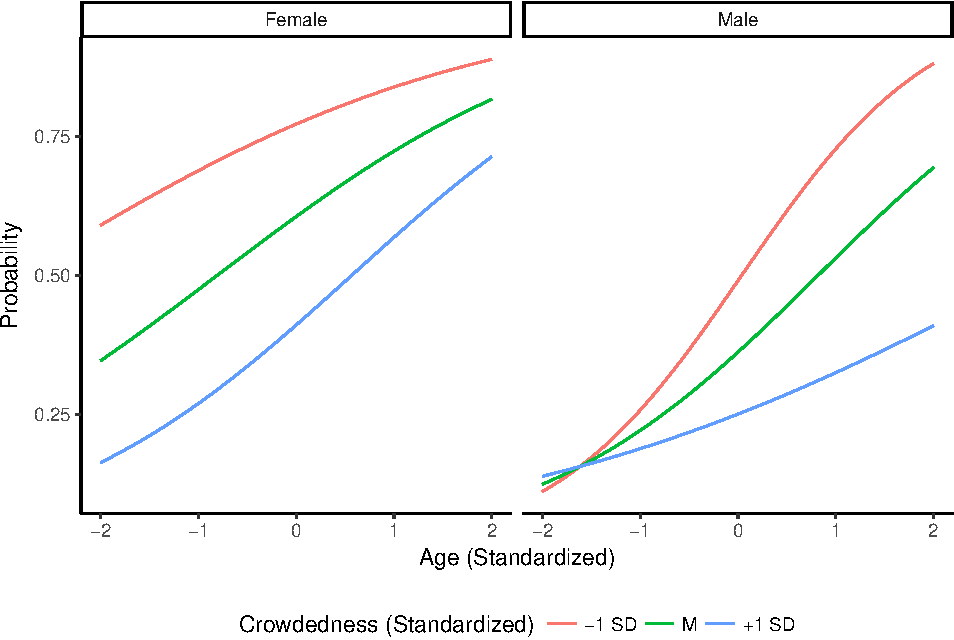
\includegraphics{Beck_HW_11_files/figure-latex/unnamed-chunk-20-1.pdf}

\subsection{Part C}\label{part-c-1}

Provide an interpretation for the plotted effect.

For young men, the probability of feeling unsafe dones't vary across
different levels of crowdedness. As they age, however, men become much
more likely to feel unsafe on uncrowded streets. Across different ages,
women are more likely to feel unsafe on less crowded streets. Older
women in general are also more likely to feel unsafe.


\end{document}
